\section{Binary Integer programming Reconfiguration problems}
\label{sec:BIP}
\subsection{Integer programming}
\begin{defn}
An integer programming problem is defined as a mathematical optimization
problem where the objective function and the constraints must be integers. 
More formally it is defined as follows :
\begin{center}
    \begin{maxi!}|l|
	  {x}{cx : Ax \leq b, x \in \mathbb{Z}^{n}}{}{}
    \end{maxi!}
\end{center}
where $A$ is an $m\timesn$ integer matrix, $c$ an $n-$dimensional row vector, $b$ an $m-$dimensional column vector and $x$ an $n-$dimensional column vector of variables or unknowns. 
\end{defn}

\begin{defn}
A binary integer programming problem also known as $0-1$ integer programming problem is an integer programming problem where $x \in \{0,1\}^{n}$. 
\end{defn}

\begin{defn}
The set of solution to the BIP is the set of vectors $V$ that satisfy all the constraints. The set $V$ is also called the set of feasible solutions. 
\end{defn}

\subsubsection{Geometry of integer programming}
\begin{defn}
Each constraint in an integer programming problem can be transformed into an equation which then represents a hyperplane in $\mathbb{R}^{n}$, a plane in $\mathbb{R}^{3}$ and a line in $\mathbb{R}^{2}$ and a point in $\mathbb{R}^{1}$ .
\end{defn}

\begin{defn}
The inequation represents one of two half spaces, which is the solution set of the inequations. A halfspace in $\mathbb{R}^{n}$ is a set of the form $\{x \in \mathbb{R}^{n} : a^{T}x \leq b\}$ for some vector a $\in$ $\mathbb{R}^{n}$ and $b \in R$.
\end{defn}

\begin{defn}
A polyhedron is the intersection of finitely many halfspaces: $P = \{x \in \mathbb{R}^{n} : Ax \leq b\}$ with edges as lines, planes, hyperplanes as the case may be.
\end{defn}

\begin{defn}
A polytope is a bounded polyhedron.
\end{defn}
\begin{example}
    \begin{maxi!}|l|
	  {}{Z = 8x_1 - 7x_2}{}{}
    \end{maxi!}
subject to : 
\begin{gather}
    x_1 + x_2 \leq 5 \\
    4x_1 + 7x_2 \leq 28 \\
    2x_1 - 3x_2 \leq 6 \\
    -3x_1 + 4x_2 \leq  12 \\
    x_1 \geq 0, x_2 \geq 0
\end{gather}
\end{example}

    \begin{figure}[H]
    \centering
    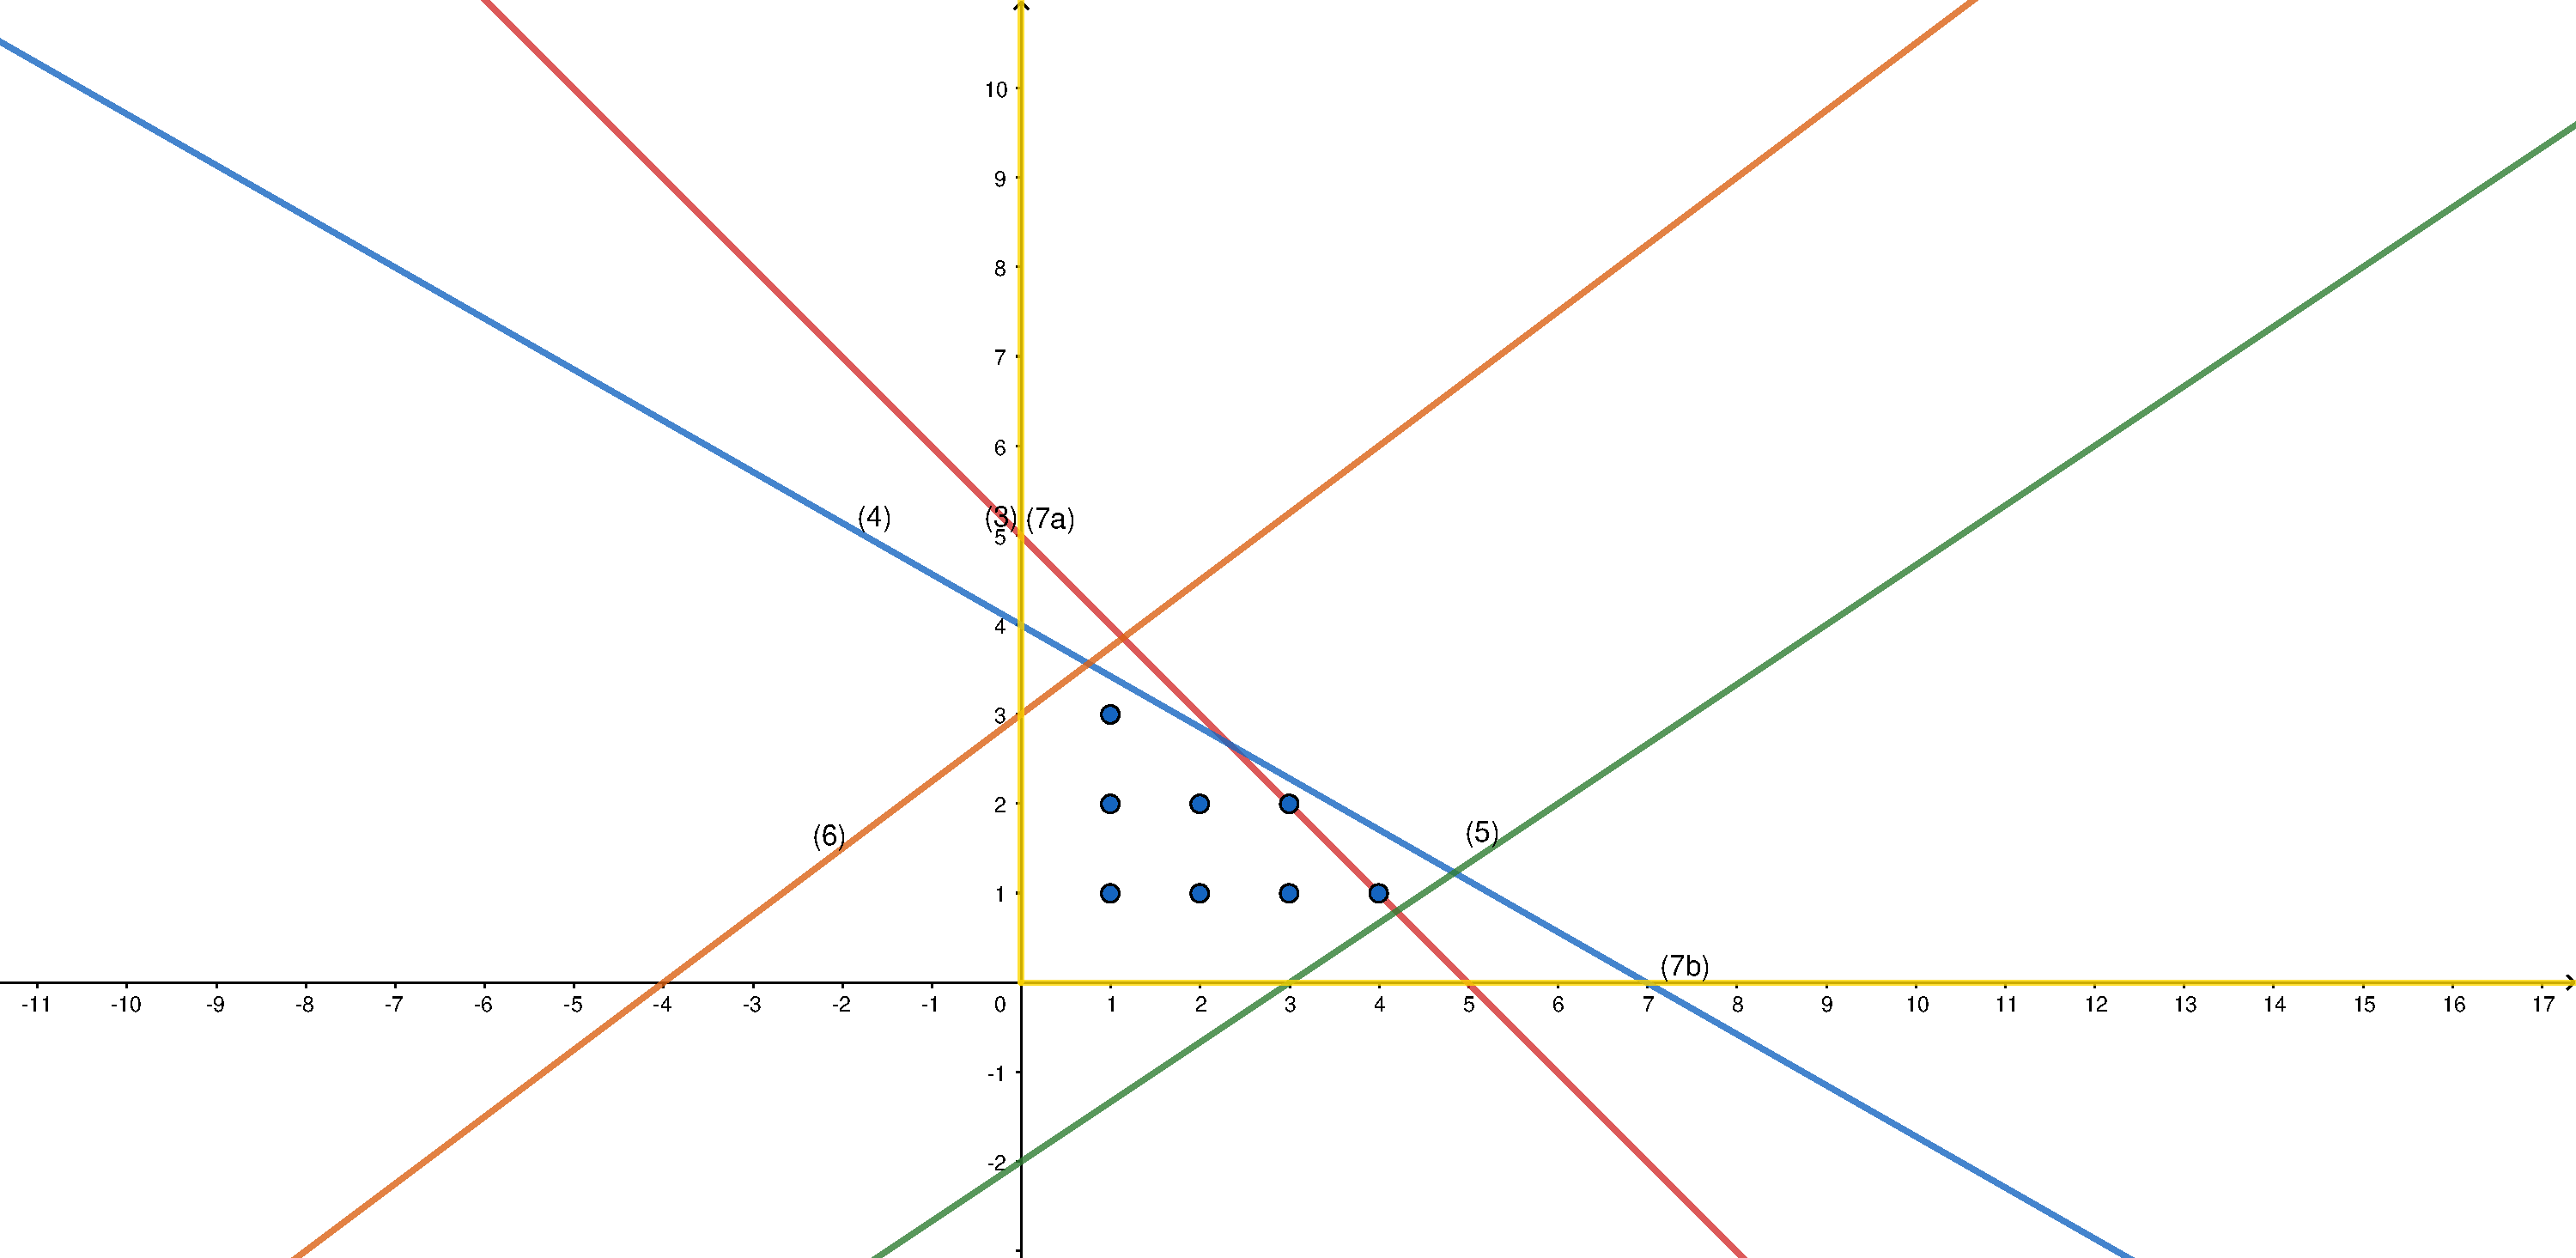
\includegraphics[width=1.0\textwidth]{res/integerp.pdf}
    \caption{Polytope yielded by the constraints of the optimization problem where the solution points correspond to the lattice points.}
    \label{fig:circle}
    \end{figure}

\subsubsection{Complexity}
\begin{theorem}
The $0-1$ integer programming problem is $\mathcal{NP}-$complete.
\end{theorem}

\begin{proof}
To prove that $0-1$ integer programming problem is $\mathcal{NP}-$complete. The two following conditions have to be satisfied : 
\begin{enumerate}
    \item $0-1$ integer programming problem is in $\mathcal{NP}$.
    \item Any problem $B$ in $\mathcal{NP}$ $\leq_{p}$ $0-1$ integer programming
    problem.\\
    The second condition can be proved by the reduction from a known $\mathcal{NP-}$complete problem.
\end{enumerate}

\paragraph{The $0-1$ integer programming problem is in $\mathcal{NP}$}.  \hfill \break
To prove that $0-1$ integer programming is in $\mathcal{NP}$ a straightforward polynomial time algorithm deciding it, is the following :  \\ 
\\
$M = $``On input $(A, b, x)$\\
1. multiply matrix $A$ with vector $x$\\
2. for $i \in (1,\ldots,m)$\\
3. ~ if $(Ax)_i > b_i$ reject\\
4. accept 

\begin{enumerate}
    \item  Multiplying each component of a row of $A$ with each component of $x$ and doing this for $m$ rows of $A$ takes $m\cdot O(n) = O(m \cdot n )$ time. 
    \item  Comparing component wise each element of $(Ax)$ with each element of $b$ makes in total $m$ comparisons is $O(m)$. 
\end{enumerate}
Final time complexity is $O(m \cdot n) + O(m) = O(m \cdot n)$ which means that $0-1$ integer programming $\in \mathcal{NP}$.

\begin{defn}
A cnf-formula is a $3$cnf-formula if all its clauses has $3$ litterals. For example  
$\phi = (x_1 \vee x_2 \vee \neg x_3) \wedge (\neg x_1 \vee x_2 \vee x_3)$. $3SAT = \{\langle \phi \rangle | \phi$  is a satisfiable Boolean formula$\} $
\end{defn}

\begin{theorem}
$3$SAT is $\mathcal{NP}$-complete.
\end{theorem}

\paragraph{$3$SAT $\leq_{p}$ $0-1$ integer programming} \hfill \break
Let $\phi$ be a $3SAT$ formula with $m$ clauses and $n$ variables. The binary integer programming instance will be constructed in the following way :  \hfill \break

For each clause in the $3SAT$ instance, we create the constraint that the sum of literals, using $z_i$ to represent $x_i$ and $(1-z_i)$ to represent $\neg x_i$, is at least 1. 
For example if $\phi=$ $(x_1 \vee \neg x_2 \vee x_3)$, the BIP instance will be constructed  as following : $z_1 + (1-z_2) + z_3 \geq 1$.  \hfill \break

To satisfy this inequality either $z_1$ should be set to $1$ or $z_2=0$ or $z_3=1$, which means we either set $x_1=true$ or $x_2=false$ or $x_3=true$ in the corresponding truth assignment.  \hfill \break

We can easily check that this construction works. \hfill \break
\begin{enumerate}
    \item Assuming that we have a satisfying assignment $S$ for $\phi$. After the construction, since $S$ is a satisfying assignment, at least one literal in each clause must be satisfied. Therefore the associated sum corresponding to constraints in the BIP instance is $\geq 1$.
    \item In the other direction, we assume we have a feasible solution to the BIP. Hence it means that each inequality must be satisfied i.e be $\geq 1$. This implies that at least one of the corresponding literal is set to $1$, since each inequality is the sum of three variables set to $1$ or $0$.
\end{enumerate}

\end{proof}

\subsection{Constrained Hypercube Path} 
The constrained hypercube path can be seen as a reconfiguration analogue to the $0-1$ Integer programming problem defined above. It is defined as follows : 

\begin{defn} \cite{cardinal_reconfiguration_2018}
Given two vertices $s,t$ of the $n-hypercube$ both be contained in a polytope $P := \{x \in \mathbb{R}^{n} : Ax \leq b\}$ for $A \in \mathbb{Z}^{d \times n}$ and $b \in \mathbb{Z}^{d}$, is there a path from $s$ to $t$ in the hypercube such that each vertices of the intermediate solution lies in $\mathcal{P}$
\end{defn}

\begin{example}
\end{example}
\begin{figure}[!h]
  \centering
  \def\svgscale{0.5}
   \def\svgwidth{width = 0.2}
  \includesvg{res/3d}
  \caption{$3$-hypercube solution space where the constraints are planes}
\end{figure}

\begin{theorem}
The constrained hypercube path problem is PSAPCE-complete, even when $d = O(1)$. \cite{cardinal_reconfiguration_2018}
\end{theorem}

\begin{proof}
The above theorem is proved by a reduction from a variant of the exact cover reconfiguration problem. It is the exact cover reconfiguration problem where more-than-2-way merges and splits are permitted. 

\begin{defn}
Exact cover problem : Given a collection $S$ of subsets of set $X$, an exact cover is the subset $S^{*}$ of $S$ such that each element of $X$ is contained is exactly one subset of $S^{*}$. It should satisfy the following two conditions : 

\begin{enumerate}
    \item The intersection of any two subsets in $S^{*}$ should be empty. That is, each element of $X$ should be contained in at most one subset of $S^{*}$.
    \item Union of all subsets in $S^{*}$ is $X$. That means union should contain all the elements in set $X$. So we can say that $S^{*}$ covers $X$.
\end{enumerate}
The Exact cover problem is a decision problem to determine if exact cover exists or not. 
\end{defn}
\begin{example}
Let $S = \{A, B, C, D, E, F\}$ and $X = \{1, 2, 3, 4, 5, 6, 7\}$ such that :\\ 
$A = \{1, 4, 7\}$ \\
$B = \{1, 4\}$ \\
$C = \{4, 5, 7\}$ \\
$D = \{3, 5, 6\}$ \\
$E = \{2, 3, 6, 7\}$ \\
$F = \{2, 7\}$ \\
Then $S^* = \{B, D, F\}$ is an exact cover, because each element in $X$ is contained exactly once in subsets $\{B, D, F\}$ . If we union subsets then we will get all the elements of $X$ – $B \cup D \cup F = \{ 1,2,3,4,5,6,7\}$
\end{example}

\begin{defn}
Exact cover reconfiguration problem : Given a collection $S$ of subsets of a set $X$ and two exact covers $C_1$ and $C_2$, can $C_1$ be reconfigured into $C_2$ via repeated splits and merges? 
\end{defn}

\begin{defn}
We could also transform an instance of the exact cover problem as a hypergraph $G = (X, S)$ where $X$ is a set and $S$ is a collection of subsets of $X$. The vertices of $G$ would be each element of $X$ and each element of $S$ is a hyperedge. 
We say that a hypergraph is $k$-colorable whenever we can assign one of $k$ colors to each vertex such that no two vertices in a hyperedge have the same color.

\end{defn}

\begin{lemma}
The exact cover reconfiguration problem is PSPACE-hard for instances that are $23$-colorable hypergraphs. \cite{cardinal_reconfiguration_2018}
\end{lemma}

\end{proof}
